\subsection{Loss-of-function constraint (gnomAD): conserved targets are constrained, CNN candidates are the least constrained set}
Conserved miRNA targets tend to be dosage-sensitive. We compared the median LOEUF (gnomAD v2.1.1 upper bound of observed/expected loss-of-function; lower means more constrained; 19,155 genes; script and results: \texttt{gnomad\_constraint}) of 200-gene sets, with the same controls fixed in advance.
Gates passed: 97.6\% of CLIP-universe genes have a LOEUF, and TargetScan conserved top-200 sets are more constrained than random UTR genes for 13/13 miRNAs ($p=1.2\times10^{-4}$). All three pre-registered CNN hypotheses are falsified, and in the opposite direction: the CNN top-200 has a higher median LOEUF than uniform random (13/13), site count (13/13) and expression-matched sets (13/13; Figure~\ref{fig:gnomad}). Not pre-registered: the two-sided sign test of this reversal gives $p=2.4\times10^{-4}$ against uniform and $p=2.4\times10^{-4}$ against expression-matched sets.
Site-count sets are more constrained than uniform random for 10/13 miRNAs, as expected if they favour genes with long 3$'$ UTRs. The CNN's preference for genes with few, strong sites may select short-UTR, less constrained genes. This post-hoc finding needs a held-out, UTR-length-matched replication before it can be read as biology, and we make no claim beyond the description.
\begin{figure}[h]\centering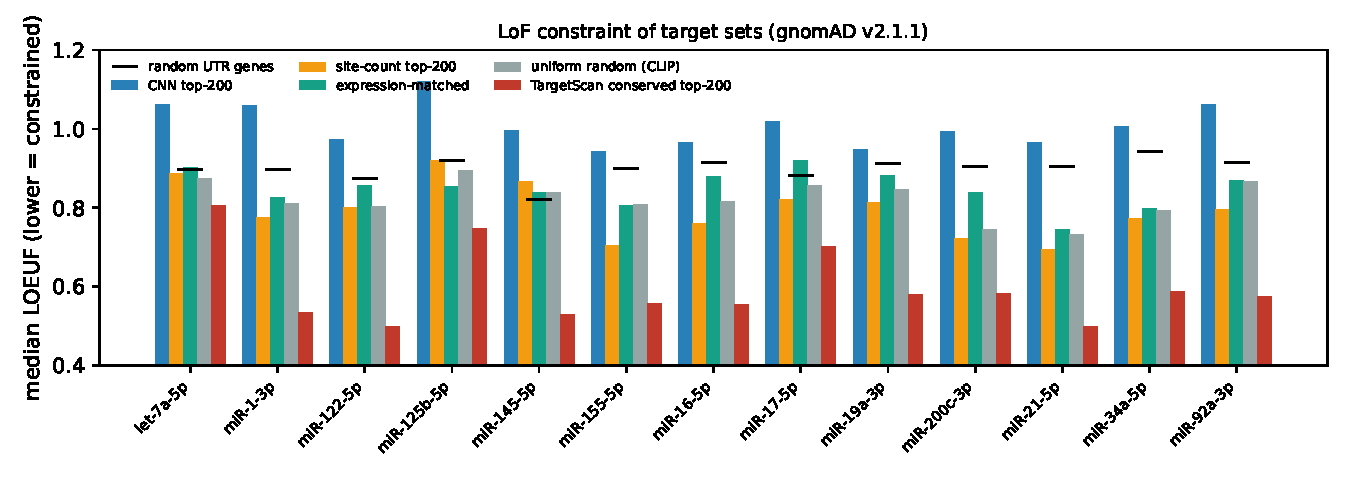
\includegraphics[width=0.95\linewidth]{figs/fig_gnomad.pdf}
\caption{Median LOEUF of each 200-gene set. Black dashes: random UTR genes, the comparator for the TargetScan positive control.}\label{fig:gnomad}\end{figure}
